\documentclass[UTF8, 11pt, a4paper]{article}
\usepackage[cm]{sfmath}
\usepackage{tabularx}
\def\arraystretch{1.3}
\usepackage[a4paper, top=3.18cm,bottom=3.81cm,left=2.54cm,right=2.54cm]{geometry}
\usepackage{indentfirst}
\setlength{\parskip}{6pt}
\XeTeXlinebreaklocale "zh"
\usepackage{graphicx}
\usepackage[normalem]{ulem}

\usepackage{fontspec}
\setmainfont{思源黑体}
\SetSymbolFont{largesymbols}{normal}{OMX}{iwona}{m}{n}
\setmonofont{Source Code Pro}

\begin{document}
\section*{木天蓼 / Matatabi}

\subsection*{描述}
Nuko 最近兴致大发,在自家的菜园里种起了木天蓼。%
这是一种神奇的植物,可以让猫咪特别兴♂奋。

木天蓼是一种长条形的植物,每一株都有一个固定的高度。%
Nuko 把它们排列在一条直线上,从左往右编号 1 至 $N$,%
并按顺序测量了每一株的高度 $h_i$。

Nuko 每天都会给木天蓼们浇水。但是 Nuko 做完那两大块蒲团之后就没有什么%
精力了,所以浇水其实就是用一个巨大的喷头——这个喷头可以喷出笔直的水平水柱%
——从整条线的左边喷一次,再从右边喷一次。聪明的 Mafu 一眼看出,第 $i$ 株%
木天蓼能得到水分当且仅当下列两条中至少一条成立:
\begin{itemize}
    \item 对于所有满足 $j \in [1, i)$ 的整数 $j$,有 $h_j \leq h_i$;
    \item 对于所有满足 $k \in (i, N]$ 的整数 $k$,有 $h_k \leq h_i$。
\end{itemize}

如果一株木天蓼长时间得不到任何水分,就会枯萎。Mafu 不想让%
它们中的任何一株枯萎,决定帮 Nuko 把它们重新排列,使得%
每一株都能得到哪怕一丁点的水分。但是这些植物对 Mafu 来说太大了,%
Mafu 每次只能交换相邻两株木天蓼。为了提前安排这项计划,Mafu 想要知道,%
为了让每株木天蓼都得到水分,所需要的最少交换次数。

\subsection*{输入 \makebox[0.5em]{} \small{matatabi.in}}
\begin{itemize}
    \item 第 1 行:一个正整数 $N$。
    \item 接下来 $N$ 行:每行包含一个正整数 $h_i$ 表示%
        从左往右第 $i$ 株木天蓼的高度。
\end{itemize}

\subsection*{输出 \makebox[0.5em]{} \small{matatabi.out}}
\begin{itemize}
    \item 第 1 行:一个正整数,表示将所有木天蓼重排列至满足条件所需的最小交换次数。
\end{itemize}

\subsection*{样例}
\begin{table}[h]\centering
\begin{tabularx}{0.8 \textwidth}{|X|X|}
\hline
\texttt{\textbf{matatabi1.in}} & \texttt{\textbf{matatabi1.out}} \\ \hline
{\ttfamily
6\newline
2\newline
8\newline
4\newline
5\newline
3\newline
6
} & {\ttfamily
3
}
\\ \hline
\end{tabularx}\end{table}
\subsubsection*{样例一 说明}
下图表示木天蓼的初始排列。

\begin{figure}[h]\centering
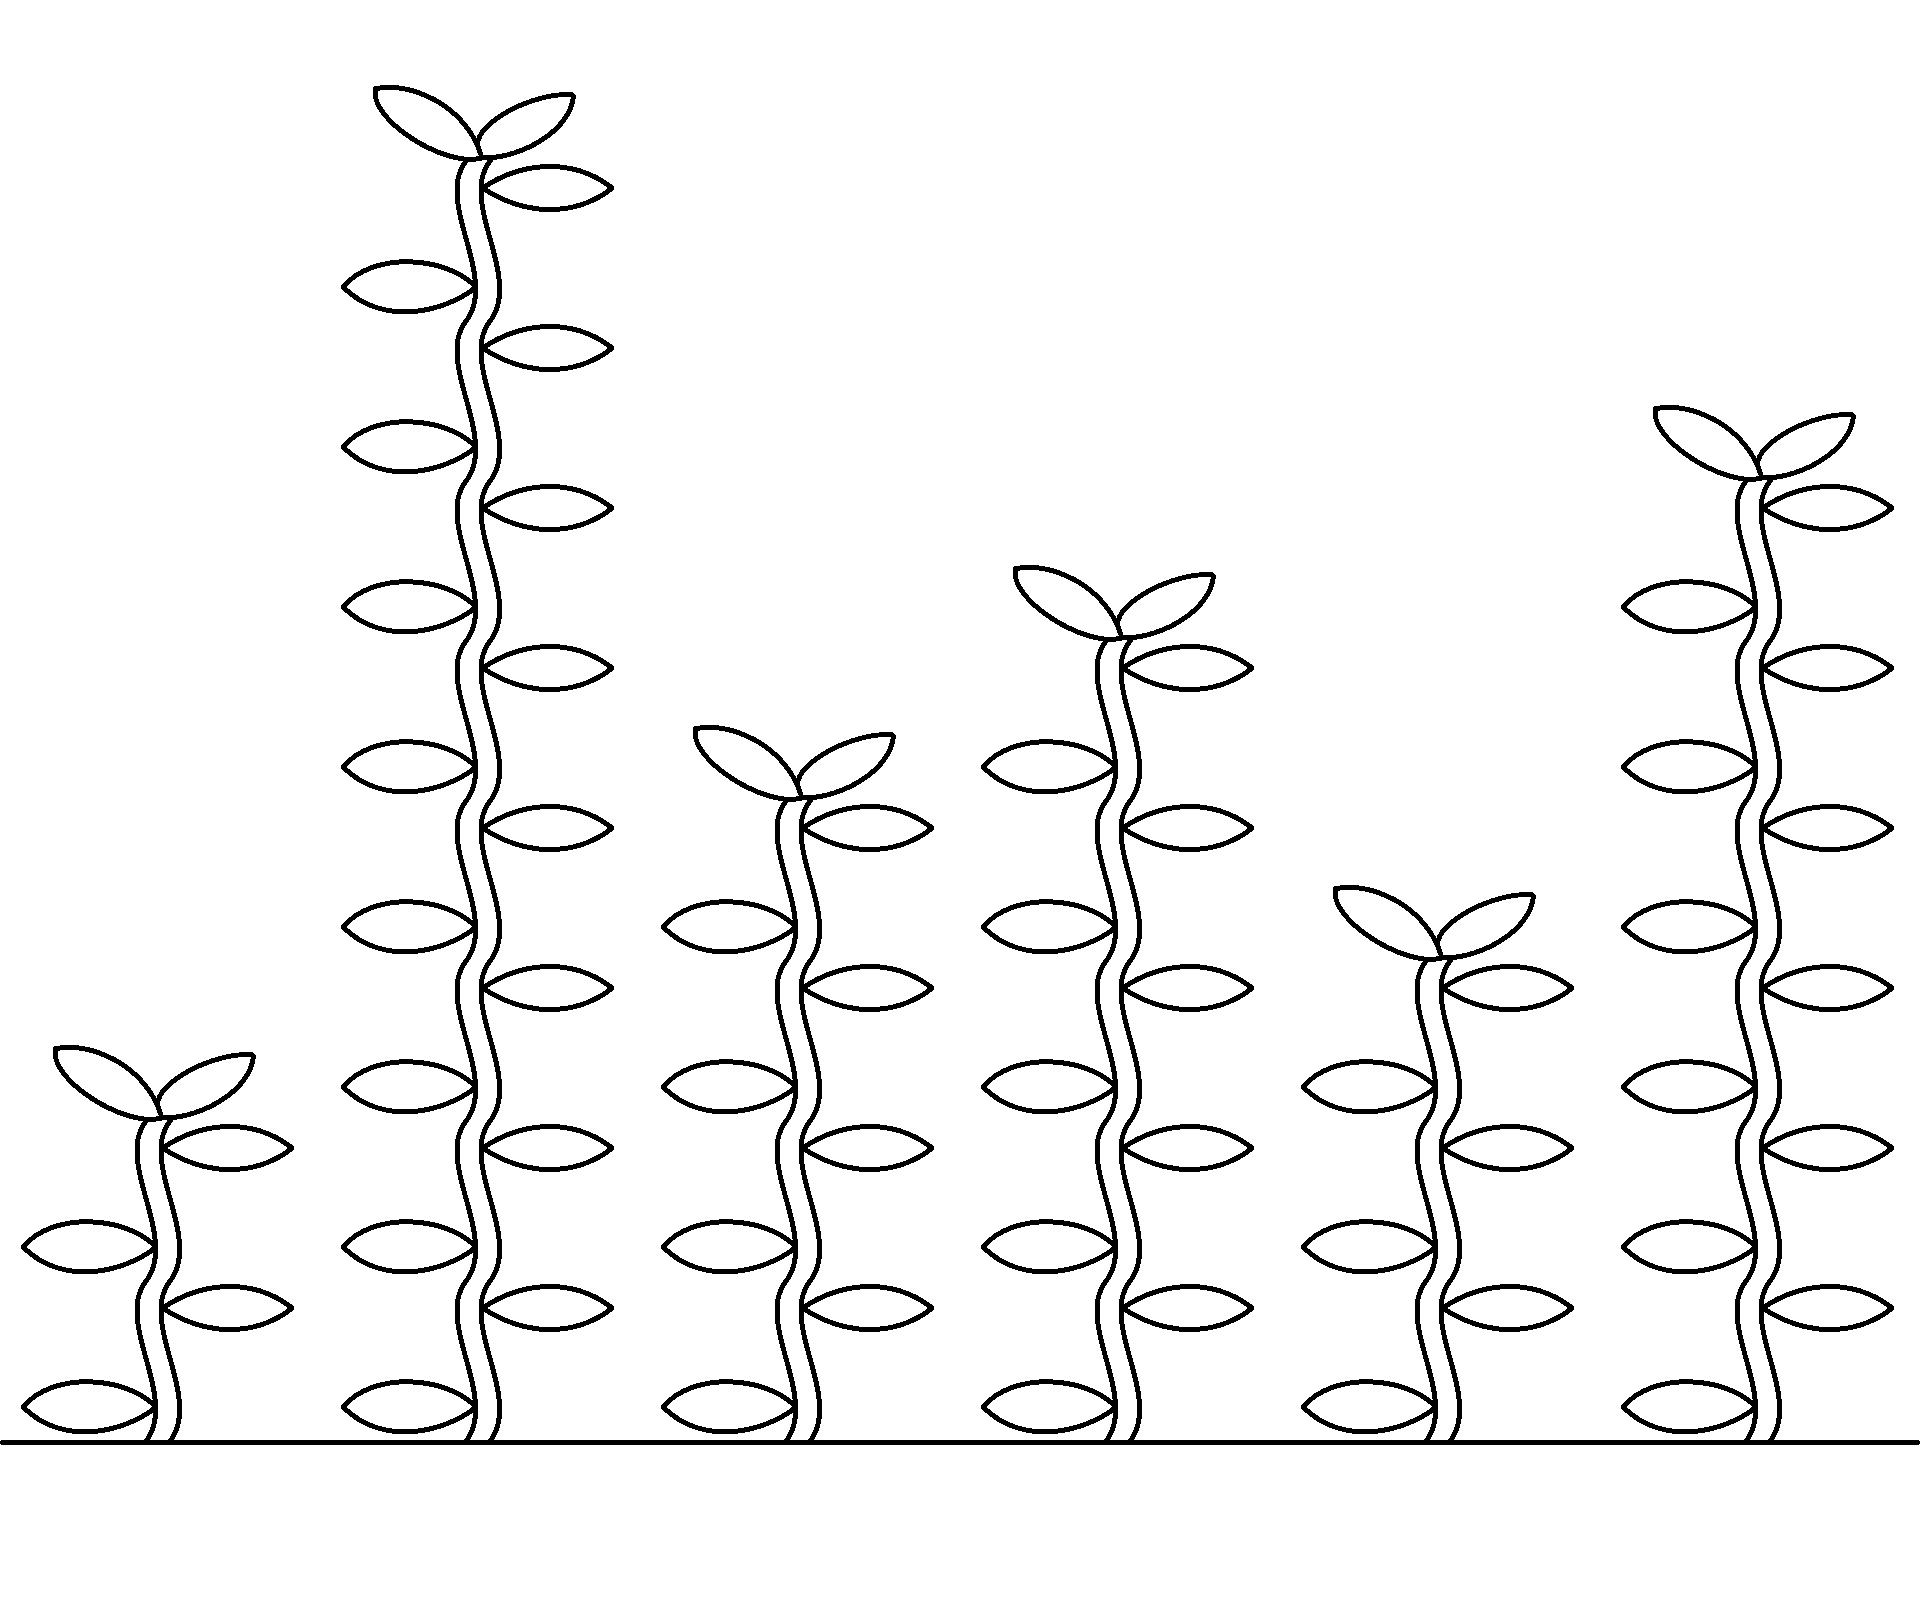
\includegraphics[width=0.45 \textwidth]{sample-1.png}
\end{figure}

按照下面的次序,可以用 3 次交换达到目标。
\begin{table}[h]\centering
\begin{tabularx}{0.9 \textwidth}{X|X}
(1) 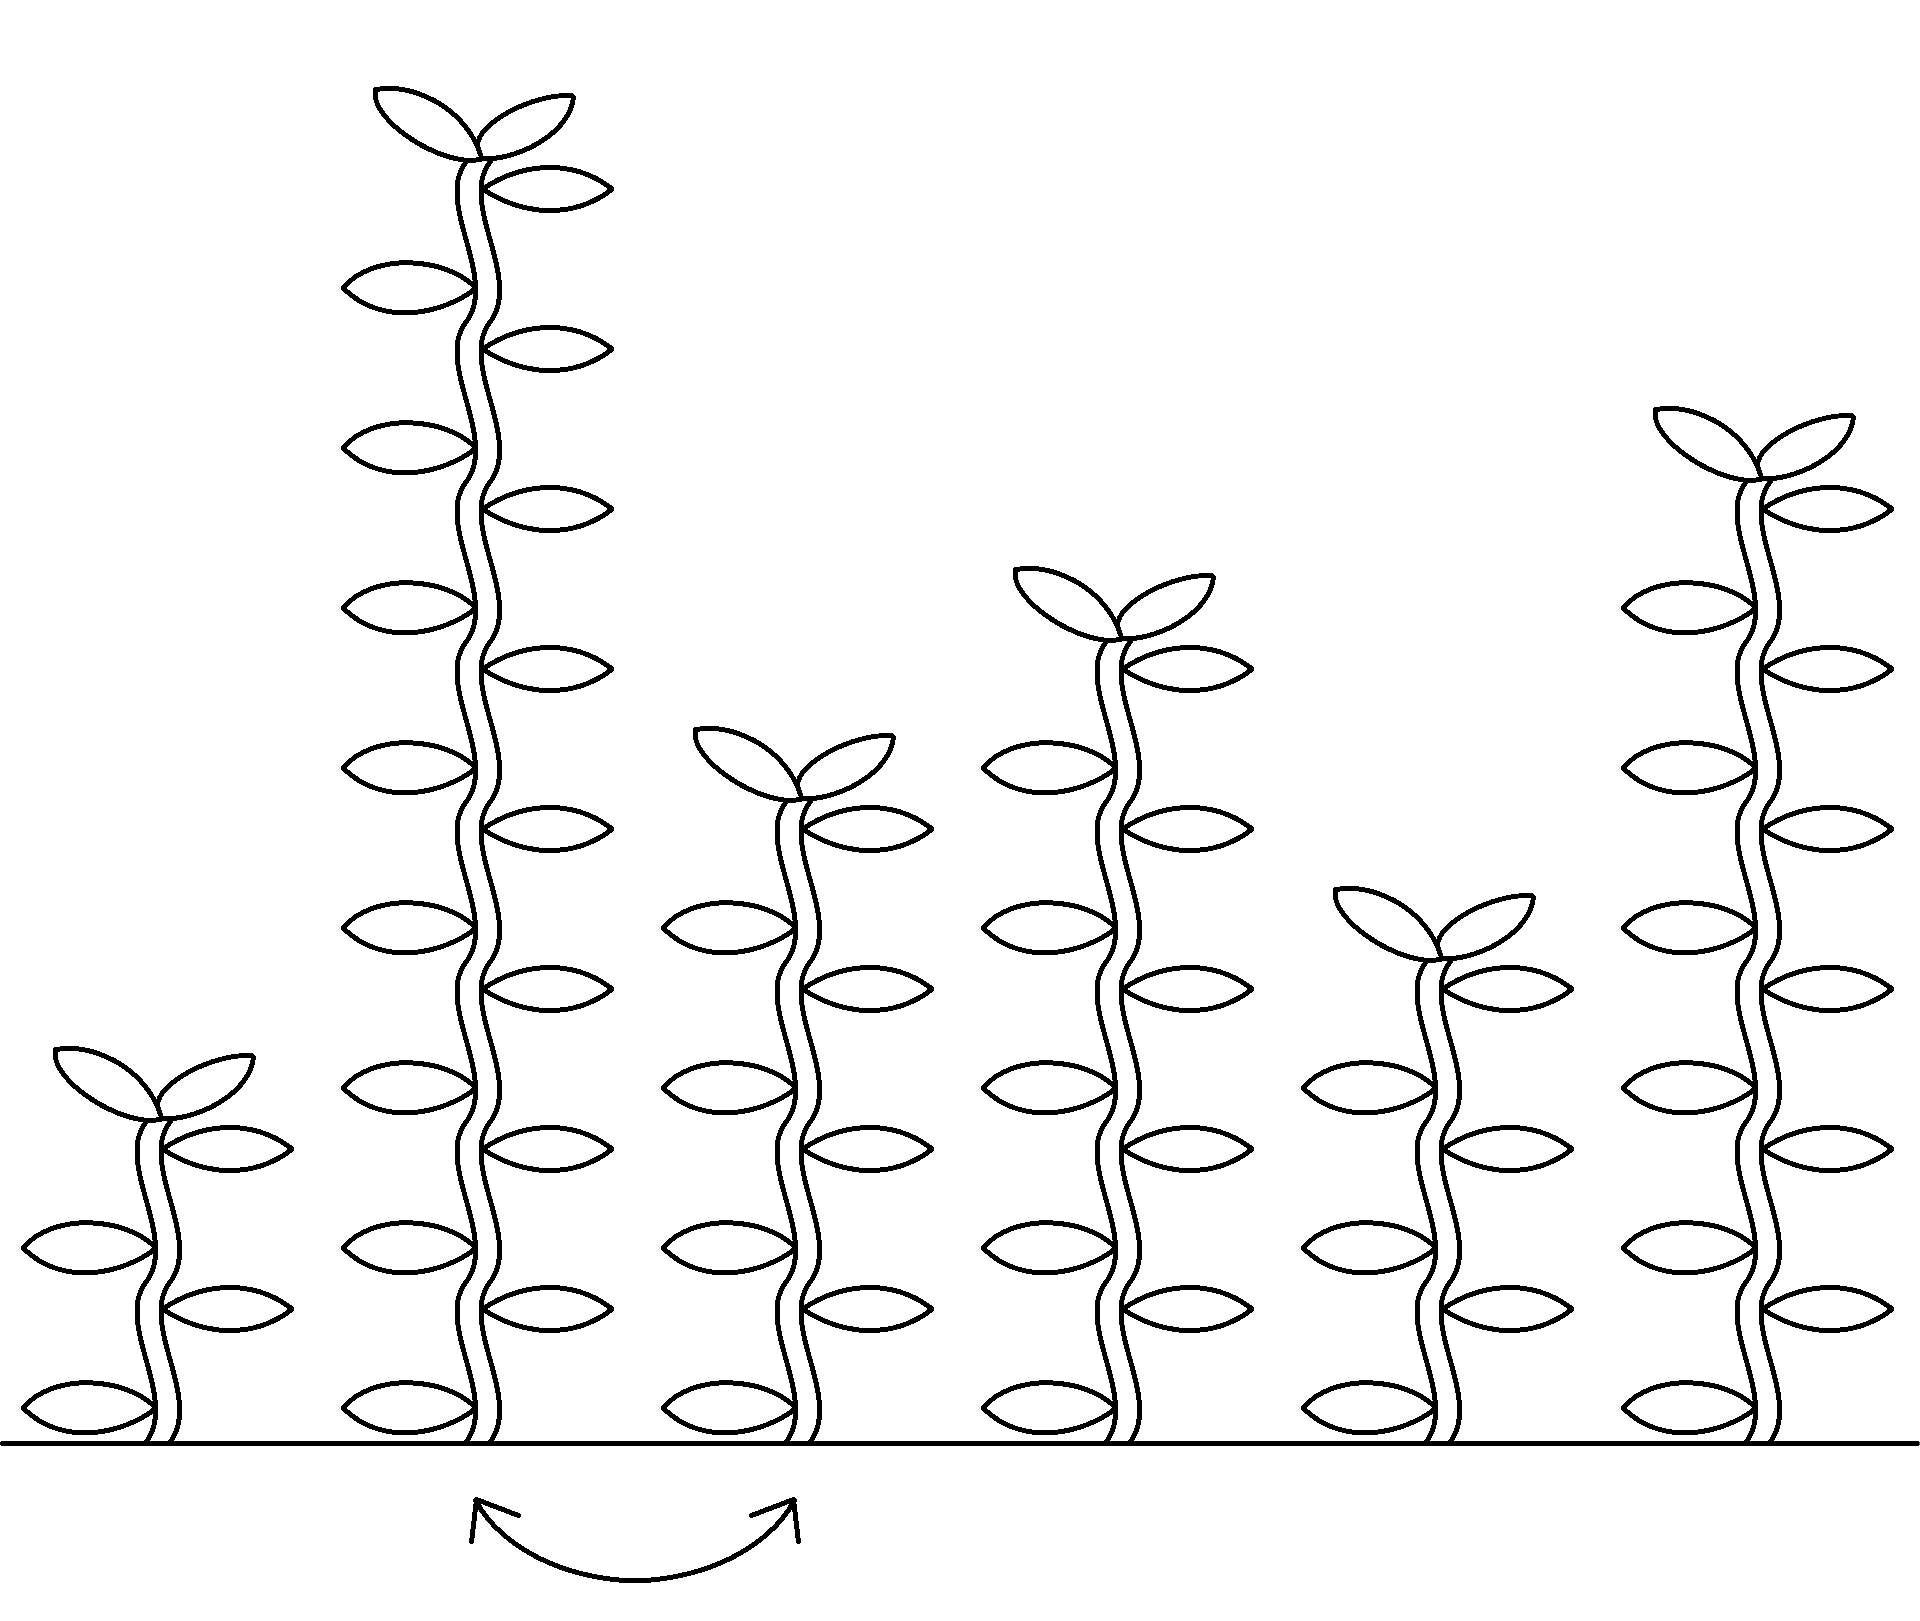
\includegraphics[width=0.37 \textwidth]{sample-2.png} &
(2) 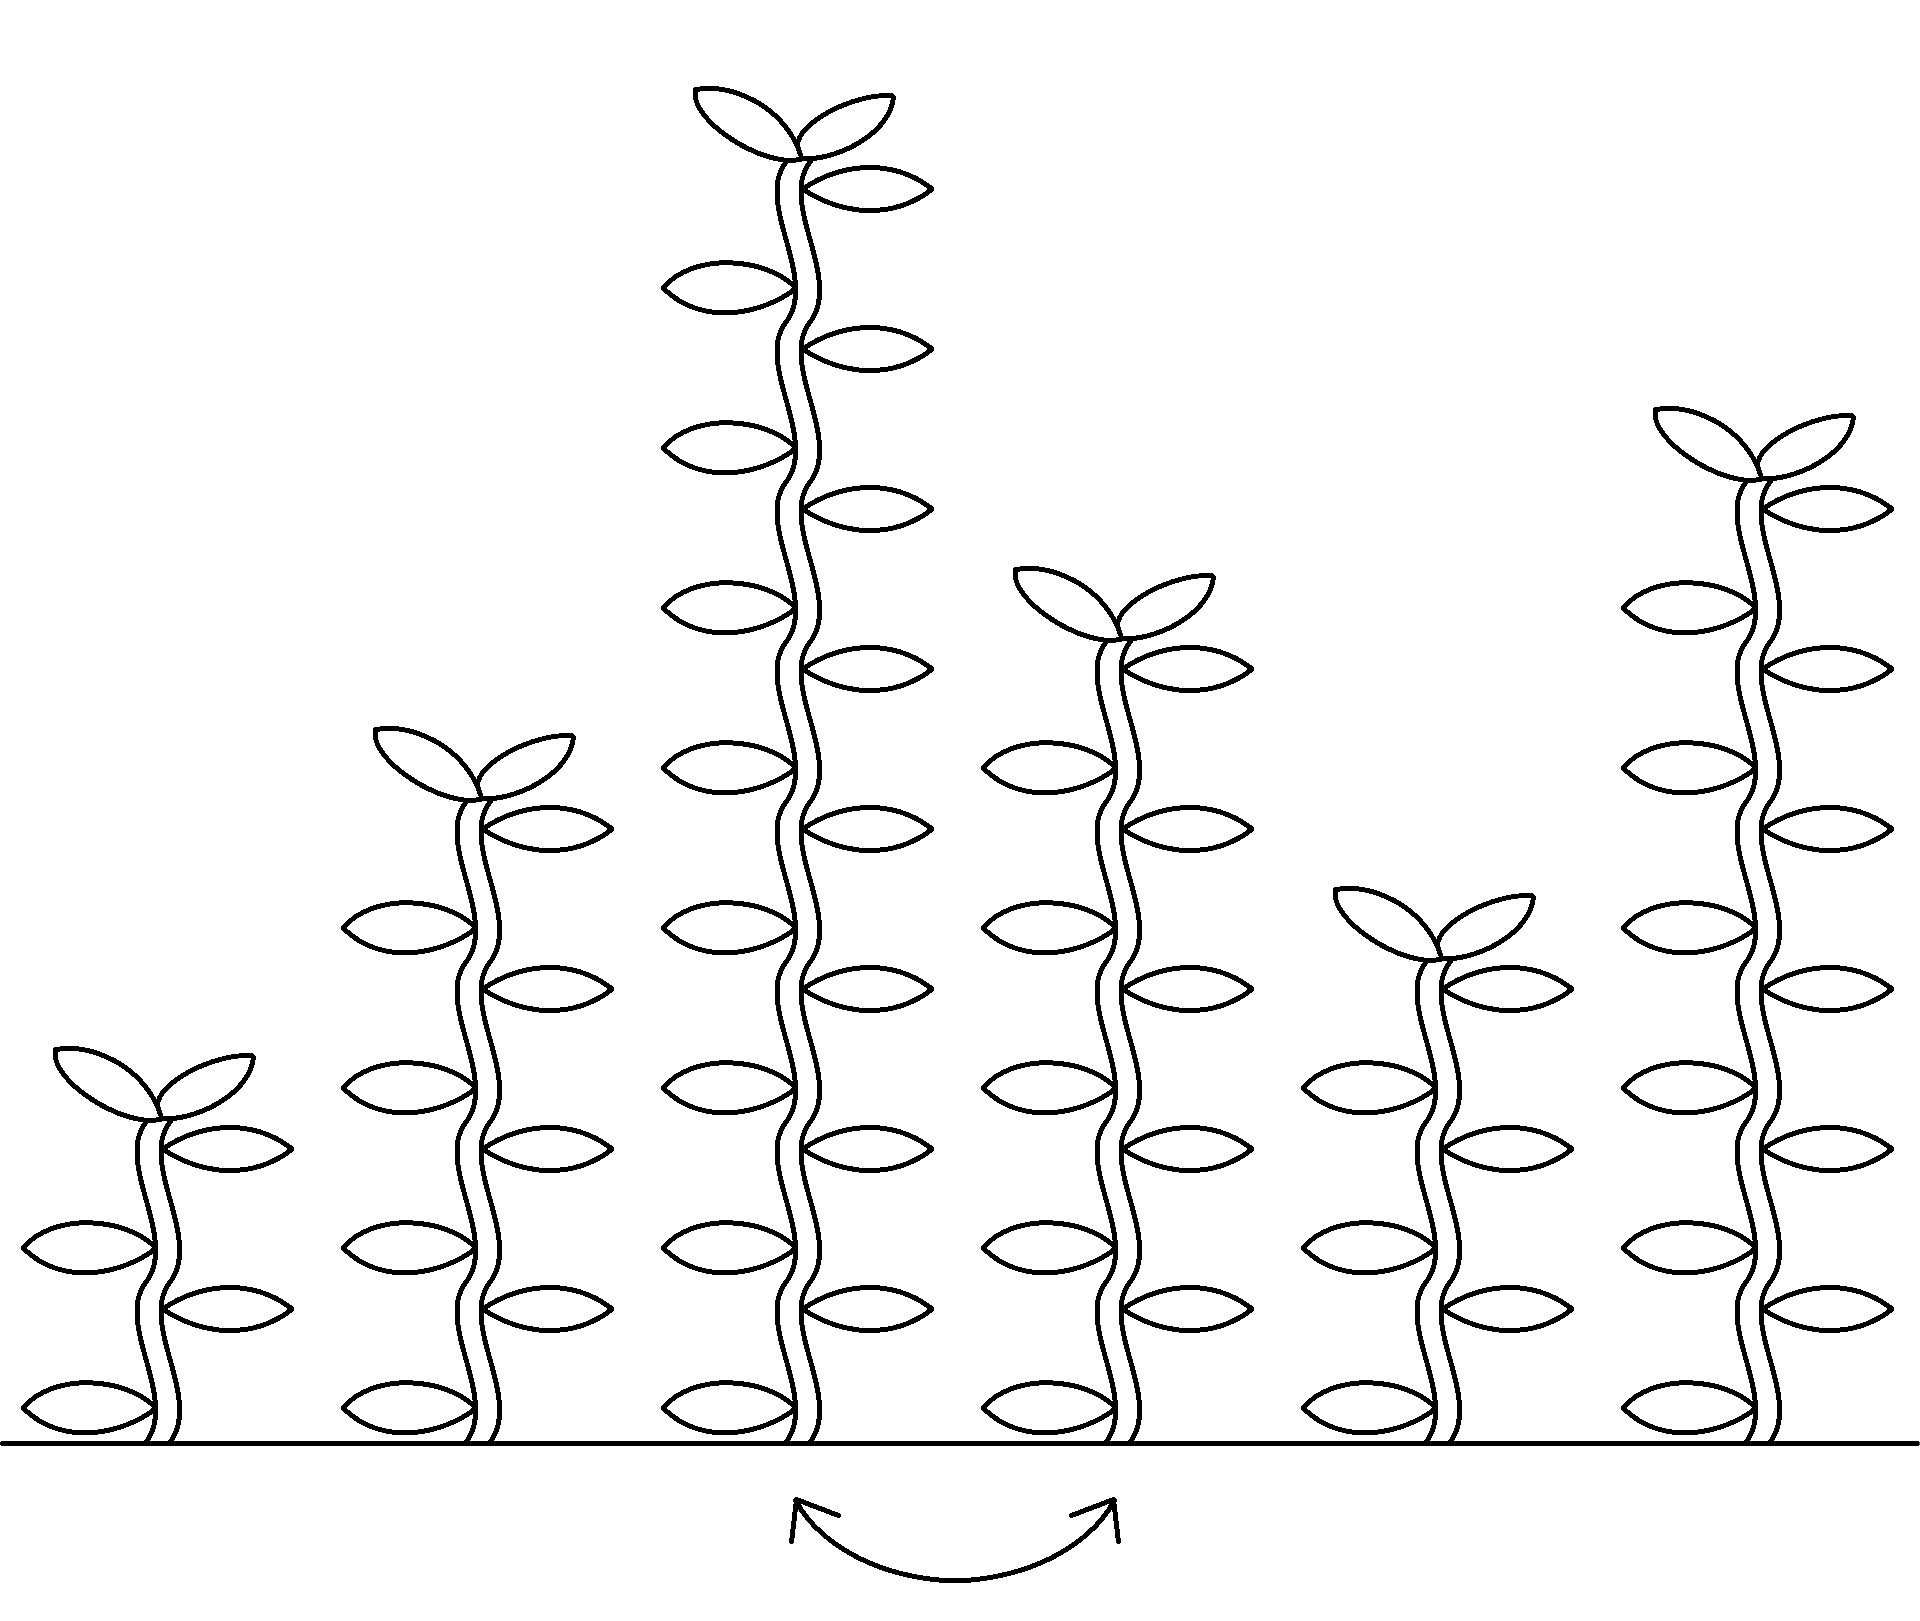
\includegraphics[width=0.37 \textwidth]{sample-3.png} \\ \hline
(3) 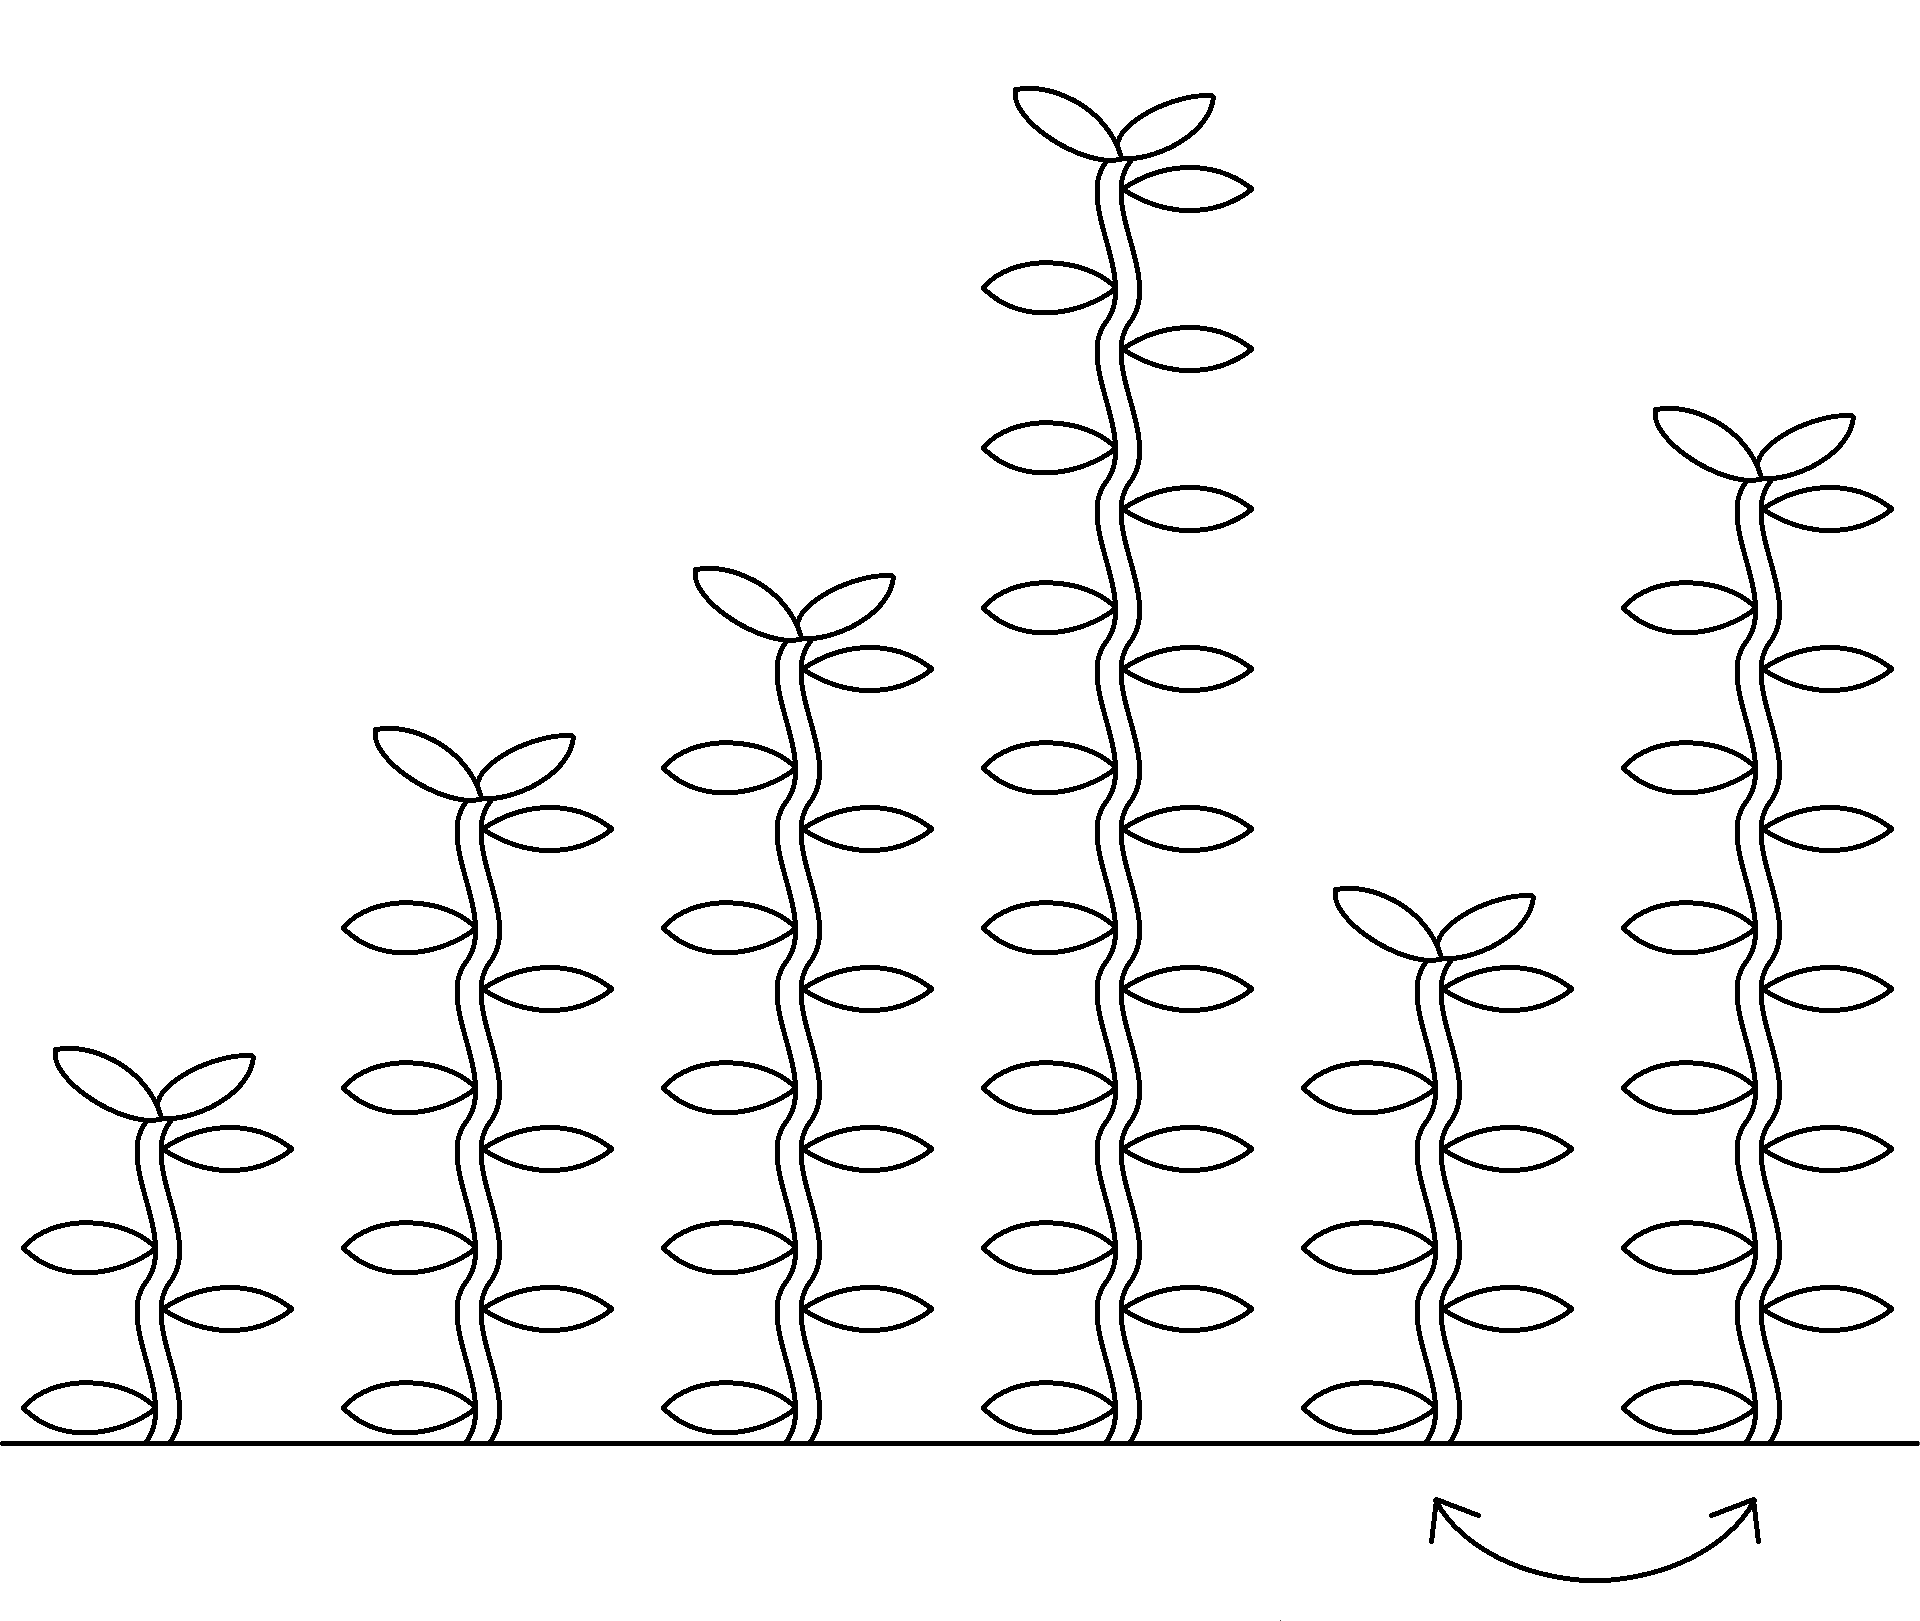
\includegraphics[width=0.37 \textwidth]{sample-4.png} &
=u= 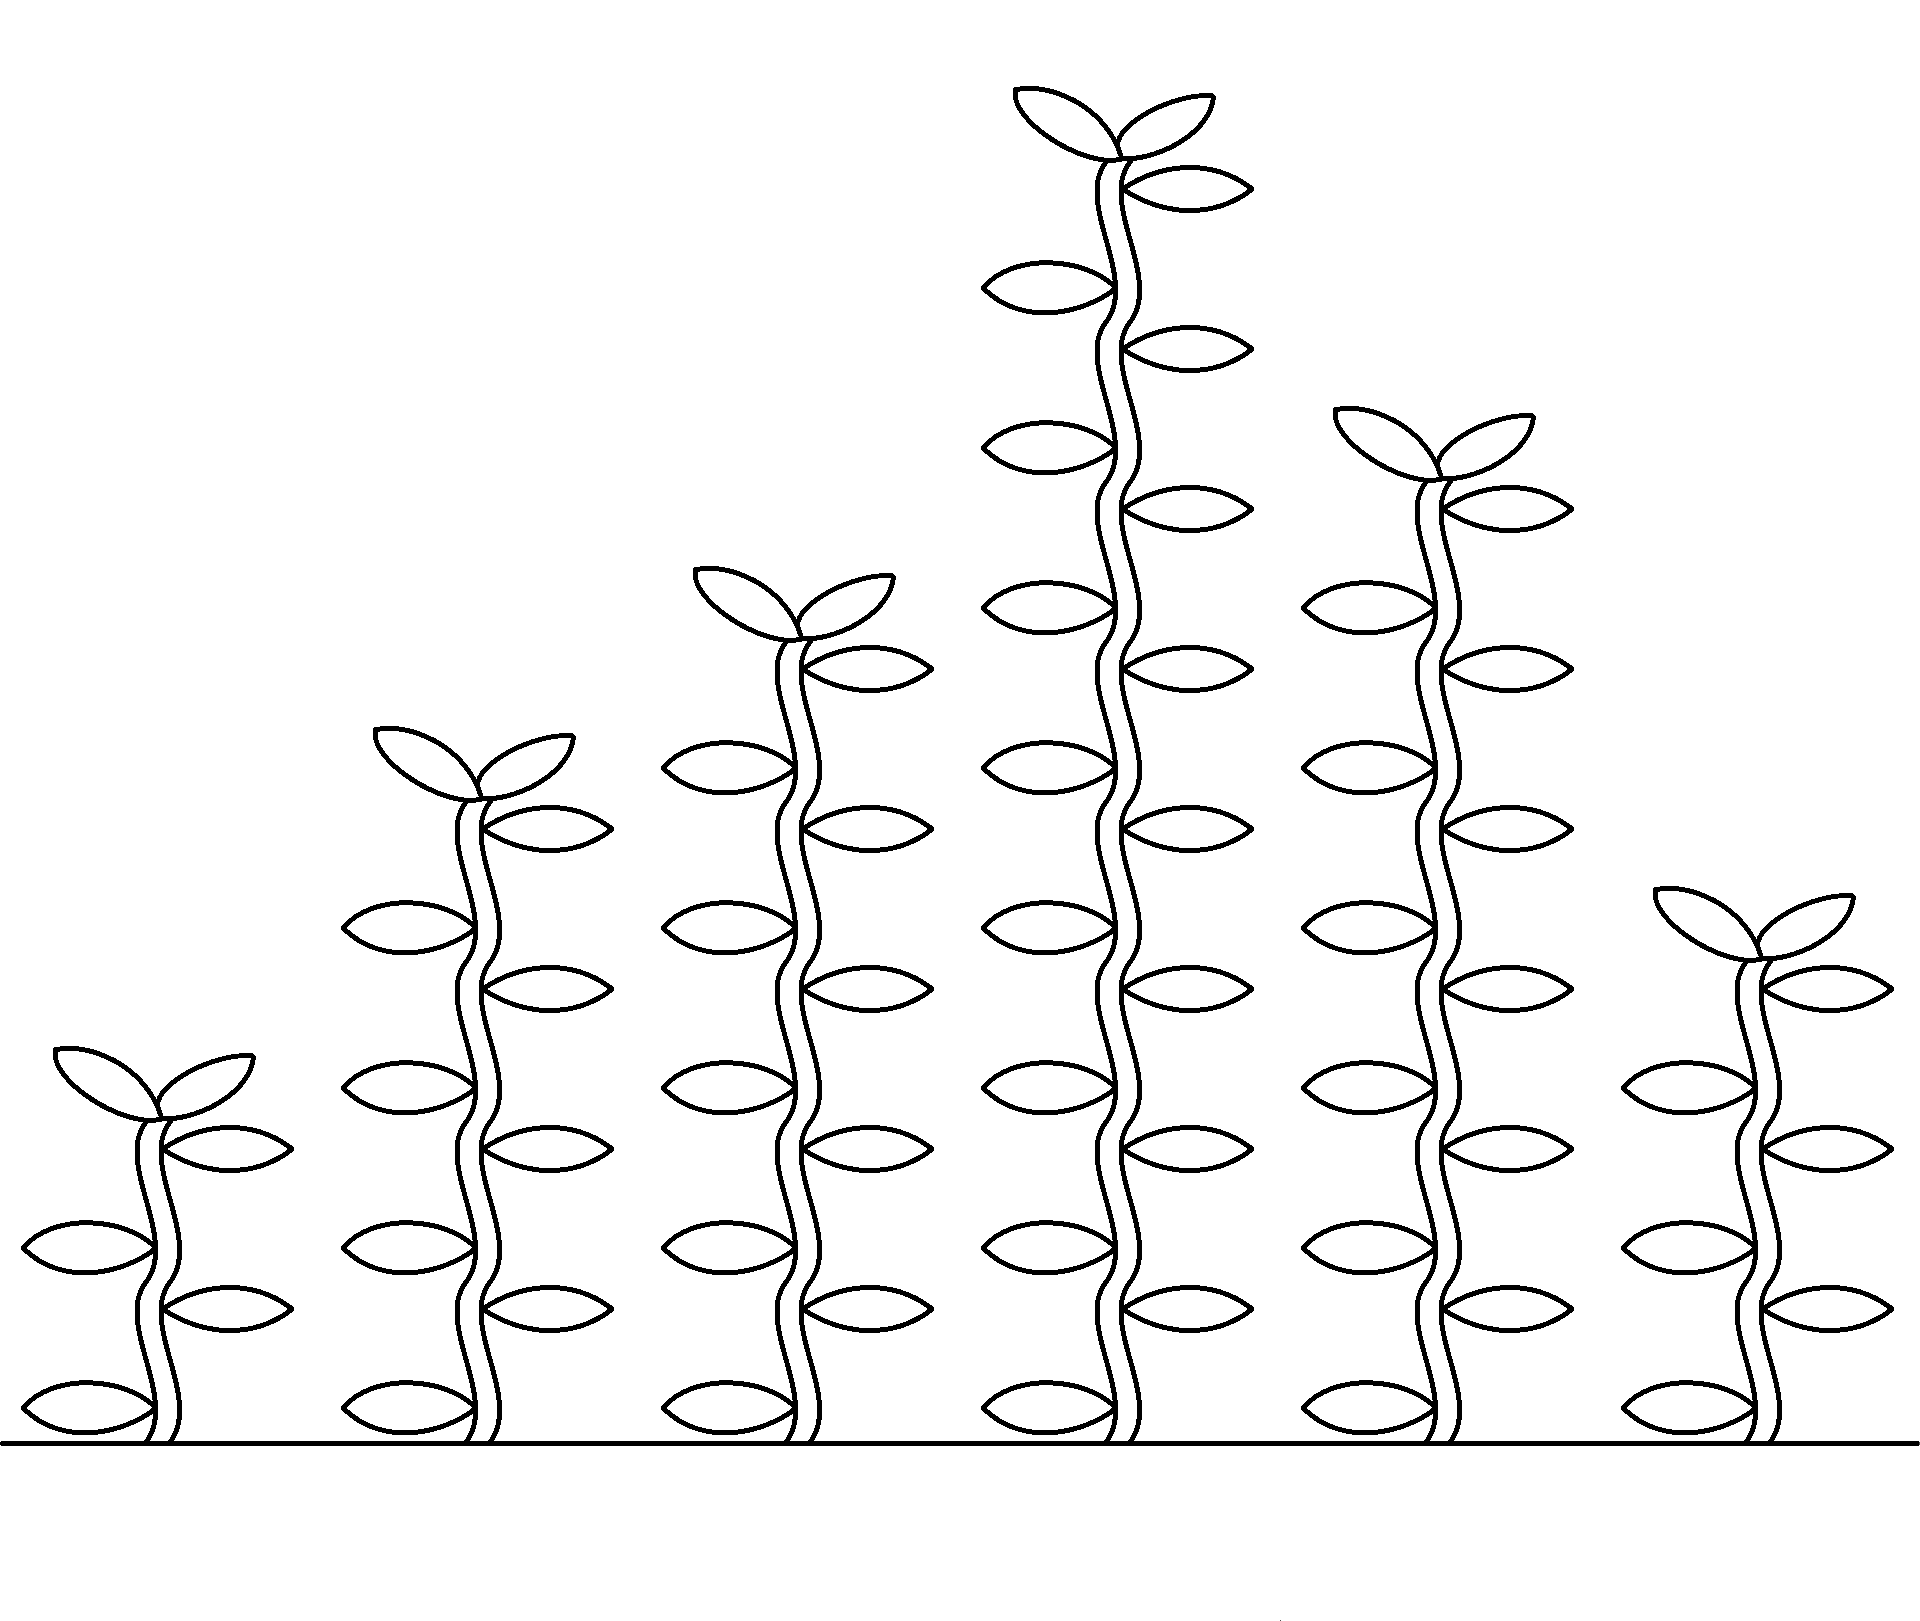
\includegraphics[width=0.37 \textwidth]{sample-5.png}
\end{tabularx}\end{table}
\newpage

\begin{table}[h]\centering
\begin{tabularx}{0.8 \textwidth}{|X|X|}
\hline
\texttt{\textbf{matatabi2.in}} & \texttt{\textbf{matatabi2.out}} \\ \hline
{\ttfamily
5\newline
4\newline
4\newline
2\newline
4\newline
4
} & {\ttfamily
2
}
\\ \hline
\end{tabularx}\end{table}
\subsubsection*{样例二 说明}
将中间的一株木天蓼用 2 次交换移动到最左边或者最右边即可。
\newline\newline

\begin{table}[h]\centering
\begin{tabularx}{0.8 \textwidth}{|X|X|}
\hline
\texttt{\textbf{matatabi3.in}} & \texttt{\textbf{matatabi3.out}} \\ \hline
{\ttfamily
4\newline
1\newline
3\newline
4\newline
2
} & {\ttfamily
0
}
\\ \hline
\end{tabularx}\end{table}
\subsubsection*{样例三 说明}
所有木天蓼原本的排列顺序已经可以保证充足的水分,不用进行交换。
\newline\newline

\subsection*{数据规模}
\begin{table}[h]\centering
\begin{tabularx}{0.75 \textwidth}{X|X|X|X}
子任务 & pts & $N$             & $h_i$       \\ \hline\hline
1      & 3   & $= 2$           & $\leq 10^9$ \\ \hline
2      & 12  & $\leq 8$        & $\leq 10^9$ \\ \hline
3      & 20  & $\leq 20$       & $\leq 10^9$ \\ \hline
4      & 20  & $\leq 5\,000$   & $\leq 10^9$ \\ \hline
5      & 27  & $\leq 300\,000$ & $\leq 300\,000$ \\ \hline
6      & 18  & $\leq 300\,000$ & $\leq 10^9$ \\
\end{tabularx}\end{table}

\subsection*{限制}
\begin{itemize}
\item 时间:1.0 秒
\item 内存:256 MiB
\end{itemize}

\begin{figure}[h]\centering

\includegraphics[width=0.6 \textwidth]{matatabi.png}
\end{figure}

\end{document}

